\let\negmedspace\undefined
\let\negthickspace\undefined
\documentclass[journal]{IEEEtran}
\usepackage[a5paper, margin=10mm, onecolumn]{geometry}
%\usepackage{lmodern} 
\usepackage{tfrupee} 

\setlength{\headheight}{1cm} 
\setlength{\headsep}{0mm}     

\usepackage{gvv-book}
\usepackage{gvv}
\usepackage{cite}
\usepackage{amsmath,amssymb,amsfonts,amsthm}
\usepackage{algorithmic}
\usepackage{graphicx}
\usepackage{textcomp}
\usepackage{xcolor}
\usepackage{txfonts}
\usepackage{listings}
\usepackage{enumitem}
\usepackage{mathtools}
\usepackage{gensymb}
\usepackage{comment}
\usepackage[breaklinks=true]{hyperref}
\usepackage{tkz-euclide} 
\usepackage{listings}
% \usepackage{gvv}                                        
\def\inputGnumericTable{}                                 
\usepackage[latin1]{inputenc}                                
\usepackage{color}                                            
\usepackage{array}                                            
\usepackage{longtable}                                       
\usepackage{calc}                                             
\usepackage{multirow}                                         
\usepackage{hhline}                                           
\usepackage{ifthen}                                           
\usepackage{lscape}
\usepackage{circuitikz}
\tikzstyle{block} = [rectangle, draw, fill=blue!20, 
    text width=4em, text centered, rounded corners, minimum height=3em]
\tikzstyle{sum} = [draw, fill=blue!10, circle, minimum size=1cm, node distance=1.5cm]
\tikzstyle{input} = [coordinate]
\tikzstyle{output} = [coordinate]




\begin{document}

\bibliographystyle{IEEEtran}
\vspace{3cm}

\title{1.2.15}
\author{AI25BTECH11009-Dasu Harshith kumar}
 \maketitle


{\let\newpage\relax\maketitle}

\renewcommand{\thefigure}{\theenumi}
\renewcommand{\thetable}{\theenumi}
\setlength{\intextsep}{10pt} 


\numberwithin{equation}{enumi}
\numberwithin{figure}{enumi}
\renewcommand{\thetable}{\theenumi}




\section*{1.2.15}
\textbf{AI25BTECH11009-Dasu Harshith kumar}

\textbf{Question 1.2.15} \\
Verify if the points 
\[
A(4,3),\quad B(6,4),\quad C(5,-6),\quad D(-3,5)
\]
are the vertices of a parallelogram.

\textbf{Solution:} \\
A quadrilateral is a parallelogram if the diagonals bisect each other, i.e., the midpoints of diagonals \( AC \) and \( BD \) are the same.

Midpoint of diagonal \( AC \):
\begin{align*}
M_{AC} &= \frac{A + C}{2} \\
       &= \frac{1}{2} \myvec{4+5 \\ 3+(-6)} \\
       &= \myvec{4.5 \\ -1.5}
\end{align*}

Midpoint of diagonal \( BD \):
\begin{align*}
M_{BD} &= \frac{B + D}{2} \\
       &= \frac{1}{2} \myvec{6+(-3) \\ 4+5} \\
       &= \myvec{1.5 \\ 4.5}
\end{align*}

Since\[
M_{AC} \ne M_{BD}
\]
the diagonals do not bisect each other.

\[
\therefore \quad A(4,3),\, B(6,4),\, C(5,-6),\, D(-3,5) \text{ do not form a parallelogram.}
\]

From the figure it is clearly verified that the theoretical solution matches with the computational solution.

\begin{figure}[H]
    \centering
    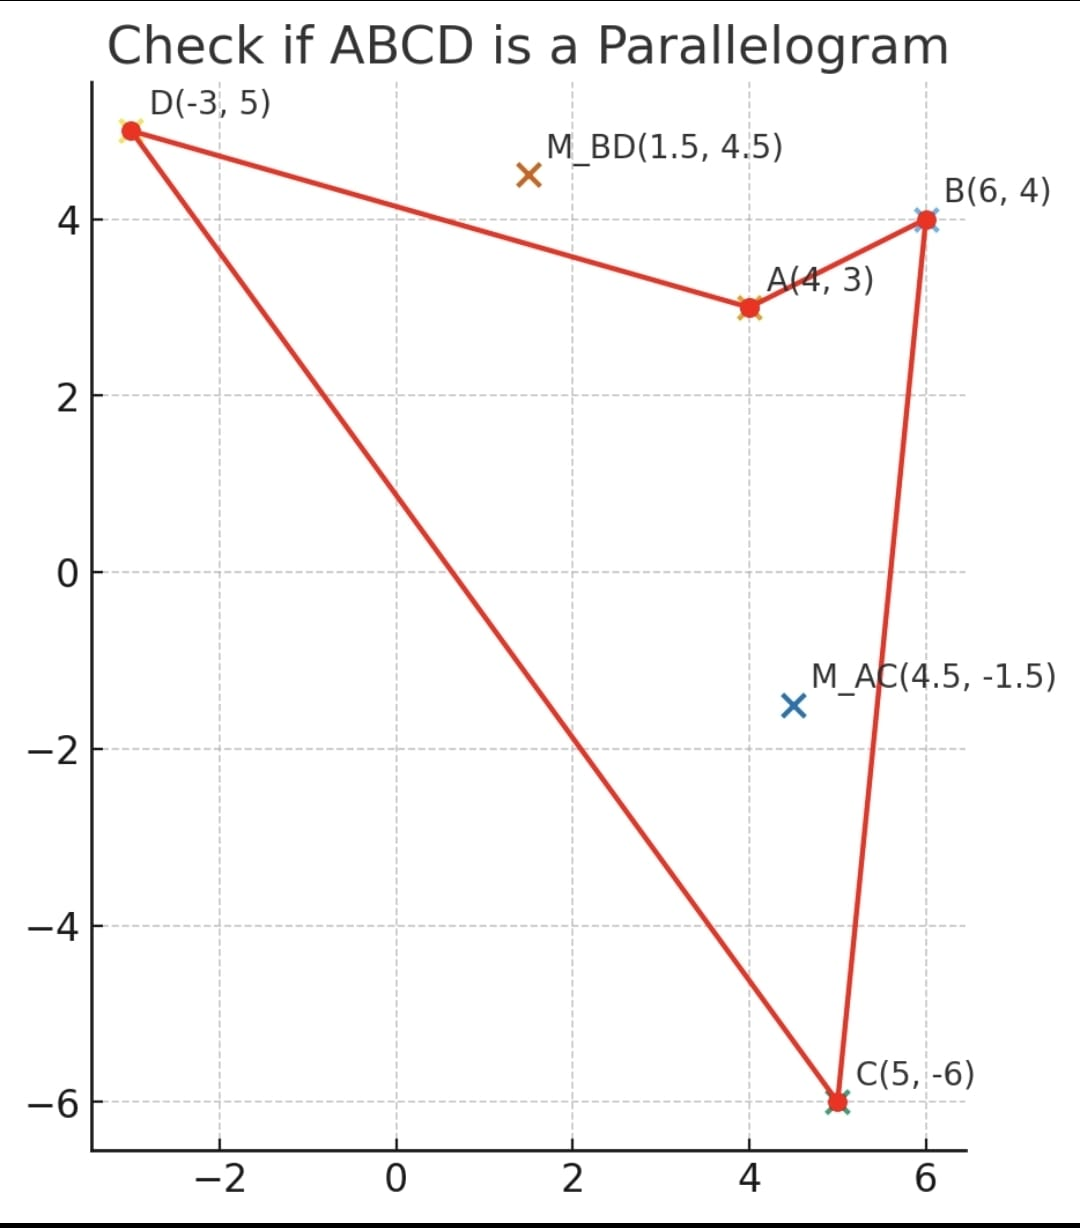
\includegraphics[width=0.7\textwidth]{figs/1_2_15.jpg}
    \caption{Plot verifying if ABCD is a parallelogram}
    \label{fig:parallelogram}
\end{figure}























\end{document}